\section{Методология}

\subsection{Данные}

Было разработано программное обеспечение, позволяющие генерировать рентгенодифракционные данные случайных органических структур (\url{github.com/blackwood168/xrd_simulator}). С помощью библиотеки CCTBX (Computational Crystallography Toolbox \cite{cctbx}) создаются кристаллические решетки, в которых случайным образом расставлены атомы, и рассчитываются структурные факторы. Также генератор поддерживает последующий расчет данных рентгеновской порошковой дифракции. Так, можно получить достоверные дифрактограммы синтетических структур, в которых реализована профильная функция Псевдо-Войдта и аксиальная расходимость пучка. Данный генератор может быть полезен для генерации рентгенодифракционных синтетических данных для использования в различных прикладных задачах машинного обучения в данной области.

Начальное обучение моделей глубокого обучения было решено проводить на синтетических данных, которые могут быть рассчитаны с помощью разработанного генератора. Высокое разрешение выбрано 0.8 Å, низкое --- 1.5 Å. Рассматриваются только симметрийно независимые отражения, так как данные о симметрии известны и без решения проблемы фаз. Так как общее количество симметрийно независимых отражений структур (для ячеек одного размера) зависит от сингонии (класса кристаллических решеток), все структуры в данных были моноклинными. Таков выбор неслучаен --- моноклинные группы симметрии являются одними из наболее распространенными для белковых структур в базе данных белков (\url{rcsb.org/stats/distribution-space-group}). Соответственно группы симметрии --- P$2_1$, C2. Типы атомов --- C, N, O, Cl; число симметрийно независимых атомов 10--30. Для обучения были сгенерированы 400.000, 100.000 и 100.000 структур для тренировочной, валидационной и тестовой выборок, соответственно.

Также в работе использовались реальные моноклинные молекулярные структуры малых молекул из Кембриджского Банка Структурных Данных \cite{csd}, для которых были расчитаны дифракционные отражения. 10.000 структур использовались для дообучения моделей на реальных структурах, 2000 --- были отложены для тестирования.

Так как отражения являются точками обратного пространства, каждое из них можно однозначно описать индексами Миллера (h,k,l). Тогда дифракционную картину можно описать трехмерным тензором, в котором записаны данные каждого отражения. Размер тензора был выбран (26,18,23) --- в матрицу такого размера помещаются все отражения для самой большой моноклинной структуры из синтетических данных. Соответственно для обучения данные об отражениях были помещены в тензор, в позициях (h,k,l) соответственно, где дифракционные максимумы отсутствуют --- стоят нули.

Для выполнения работы валидным является предсказание как интенсивности, так и амплитуды структурных факторов ($|F| = \sqrt{I}$). Типичные распределения этих данных для сгенерированных структур представлены на рис. \ref{F_dist}. Как можно заметить, распределение амплитуд больше похоже на стандартное, поэтому именно амплитуды были выбраны для решения задачи. Дифракционные данные также были отнормированы в диапазон 0-1.

\begin{figure*}[ht!]
            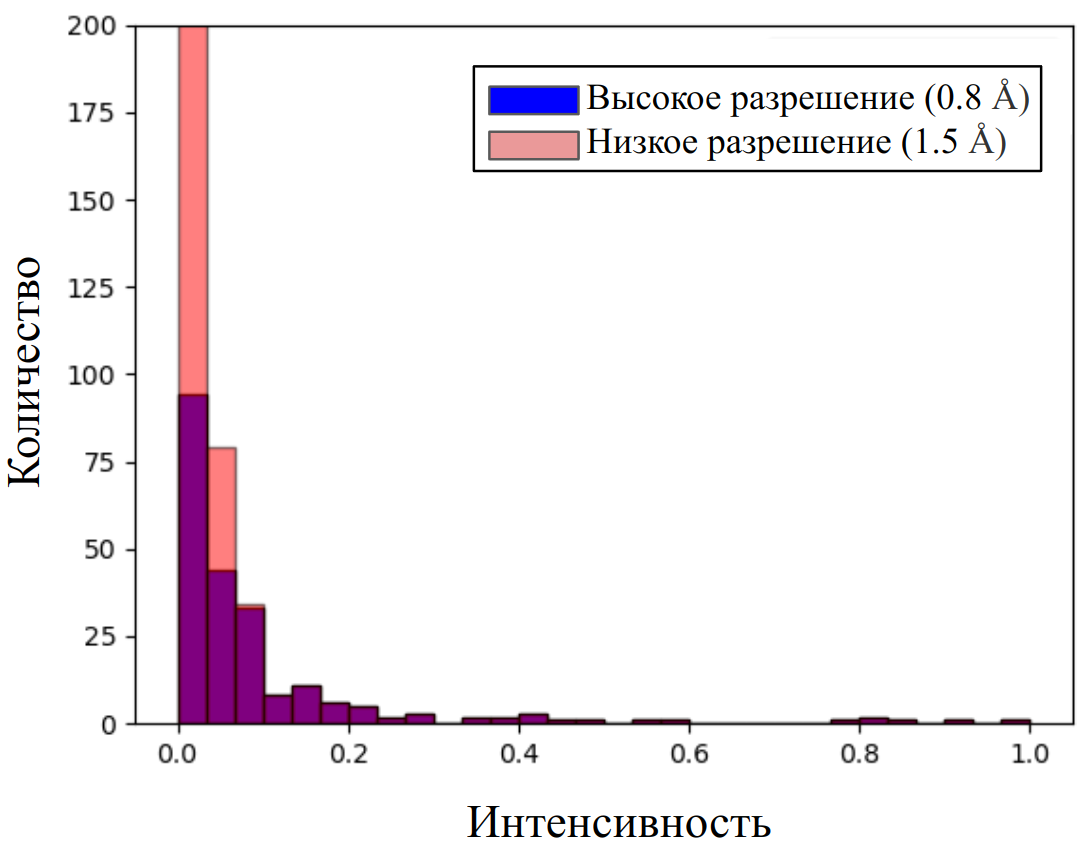
\includegraphics[width=.5\textwidth]{figures/F2_distribution.png}\hfill
            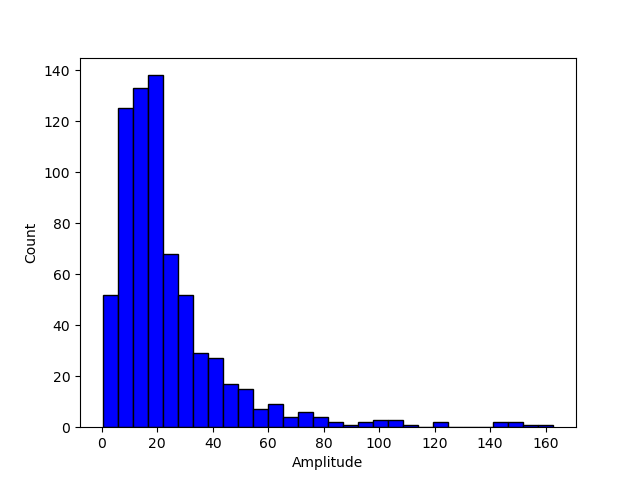
\includegraphics[width=.5\textwidth]{figures/F_distribution.png}
            \caption{Типичные распределения интенсивностей (слева) и амплитуд (справа) дифракционной картины}
            \label{F_dist}
\end{figure*}

Основная же сложность работать с чистыми амплитудами структурных факторов --- то есть с точками в обратном пространстве --- заключается в том, что данные не являются локально связанными, как изображения (рис. \ref{locally}). Это вносит специфику в данную задачу и создает трудности, так как типичные архитектуры моделей для работы с трехмерными данными, например, видео или медицинскими данными \cite{mrt} могут не сработать.

\begin{figure*}[ht!]
            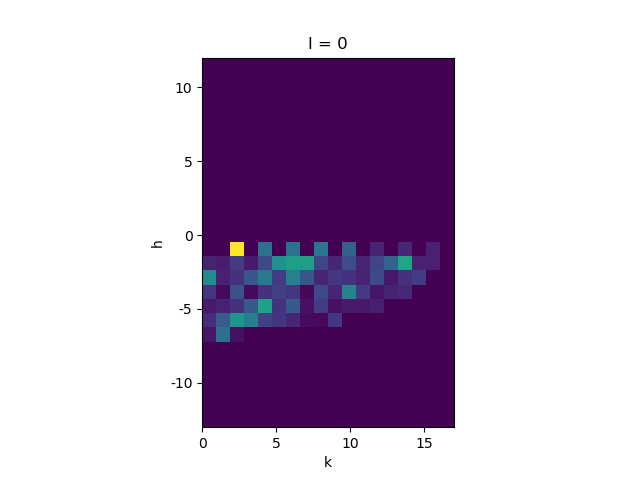
\includegraphics[width=.3\textwidth]{figures/hk_plane_l_0.png}\hfill
            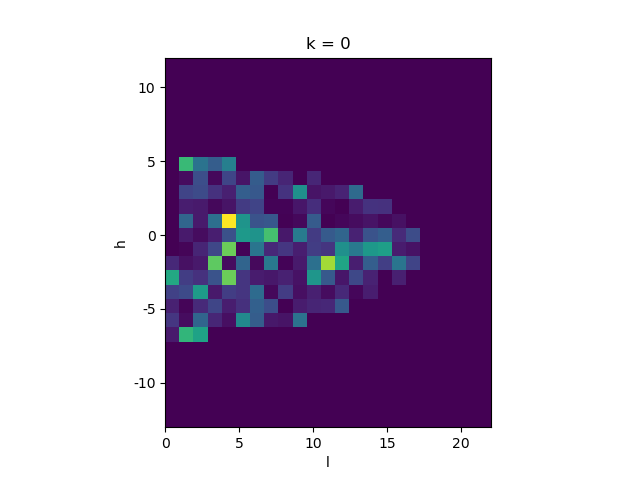
\includegraphics[width=.3\textwidth]{figures/hl_plane_k_0.png}\hfill
            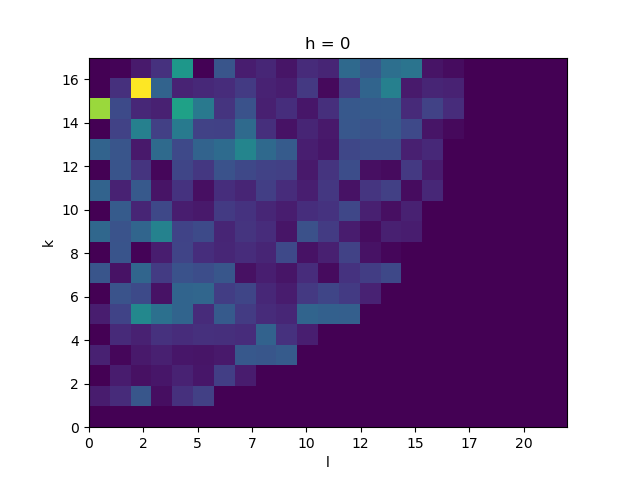
\includegraphics[width=.3\textwidth]{figures/kl_plane_h_0.png}
            \caption{Типичные сечения тензора отражений для реальных структур из CSD}
            \label{locally}
\end{figure*}

\subsection{Методы}

 работе было предложено предсказывать амплитуды дифракционных отражений белков, которые нельзя получить из эксперимента, по известным из того же эксперимента. После предсказания достаточного количество рефлексов, разрешения должно хватить для определения фаз и расчета электронной плотности одним из рутинных ab initio методов, в качестве которого был выбран SHELX \cite{shelx}.

Таким образом, задача сводится к восстановлению трехмерного тензора. Inference моделей глубокого обучения должен выглядеть следующим образом: на вход подается тензор с рентгенодифракционными экспериментальными данными, на выходе должен быть тензор с дополнительными интенсивностями. В ходе обучения планируется научить модель восстанавливать тензор отражений по данным малых органических молекул. Для этого будут обнулены интенсивности дальних отражений так, чтобы длина разрешения полученной дифракционной картины соответствовала типичному разрешению белковых соединений (1.5 Å).

В качестве baseline была обучена модель UNet, адаптированная для трехмерных тензоров (рис. \ref{unet}). Данная модель выбрана потому что она хорошо себя проявляет в простейших задачах Super Resolution, однако в данной задаче она не достигнет высокой точности из-за локальной несвязанности рентгенодифракционных данных. 

\begin{figure}[H]
    \centering
    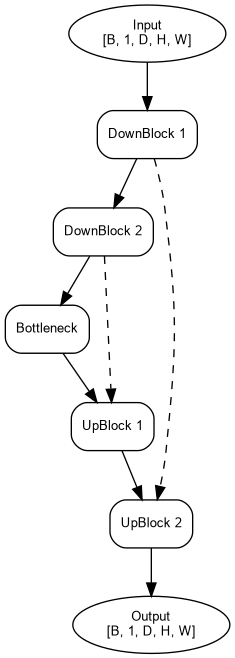
\includegraphics[width=0.25\textwidth]{figures/mini_unet_architecture.png}
    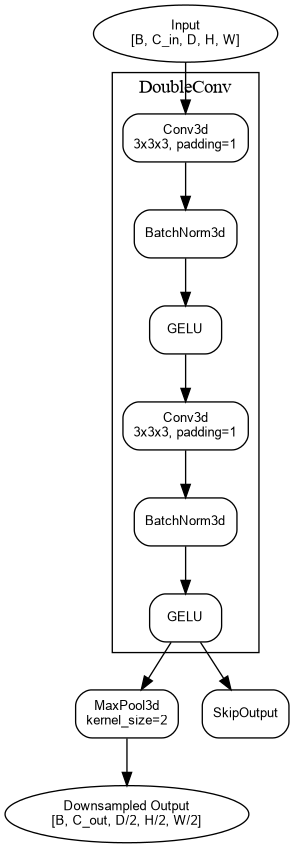
\includegraphics[width=0.25\textwidth]{figures/downblock_architecture.png}
    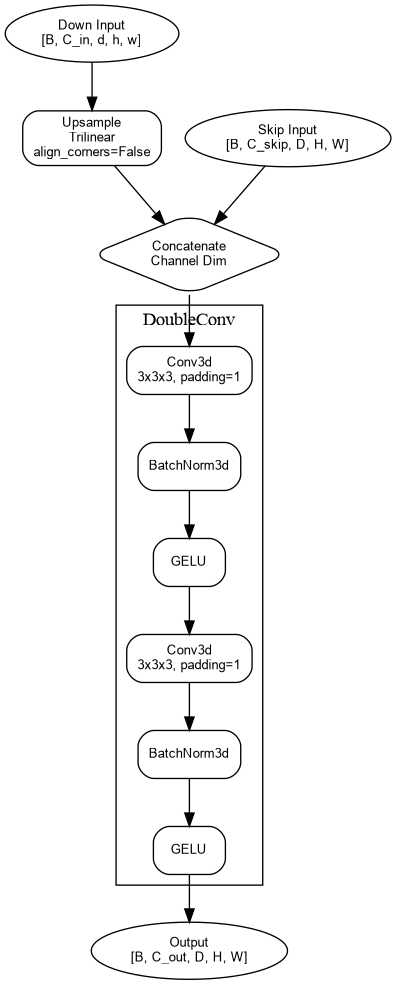
\includegraphics[width=0.3\textwidth]{figures/upblock_architecture.png}
    \caption{Схемы архитектуры модели UNet (слева) и её DownBlock(посередине) и UpBlock(справа)}
    \label{unet}
\end{figure}

Также была разработана и обучена UNet-like модель с кастомными слоями, содержащими Фурье-преобразование (рис. \ref{fft_unet}). Данный подход был продемонстрирован в работе \cite{fft} при работе с дифракционными данными и он является многообещающим и для нашей задачи, поскольку при переходе в прямое пространство наши данные являются локально связанными.


\begin{figure}[H]
    \centering
    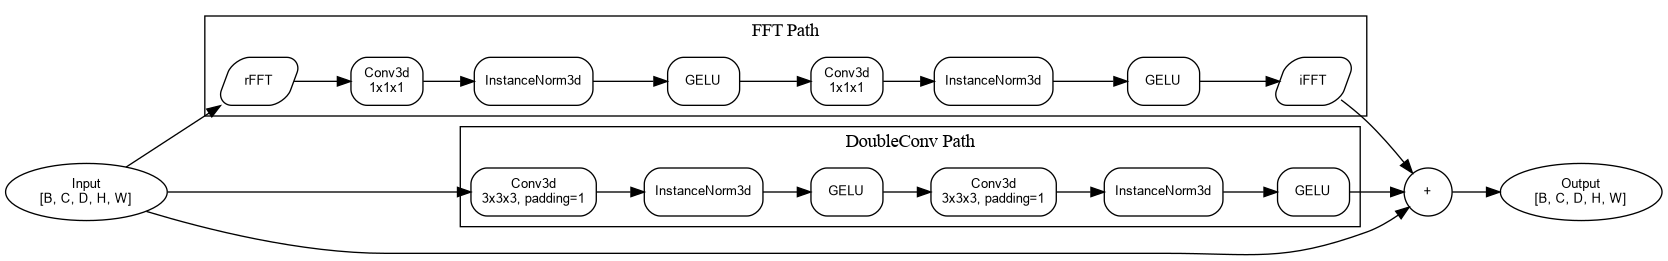
\includegraphics[width=0.8\textwidth]{figures/resf_block_architecture.png}
    \caption*{(a) Кастомный слой с Фурье-преобразованием}
    
    \vspace{1em}
    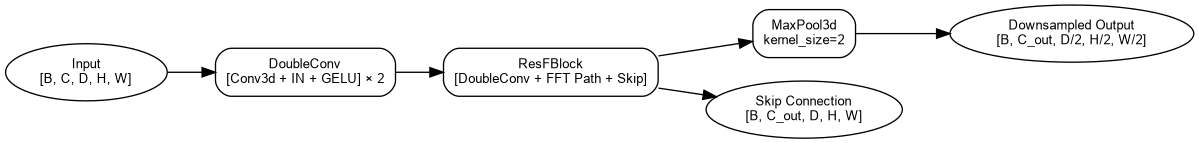
\includegraphics[width=0.8\textwidth]{figures/fft_down_block_architecture.png}
    \caption*{(b) DownBlock}
    
    \vspace{1em}
    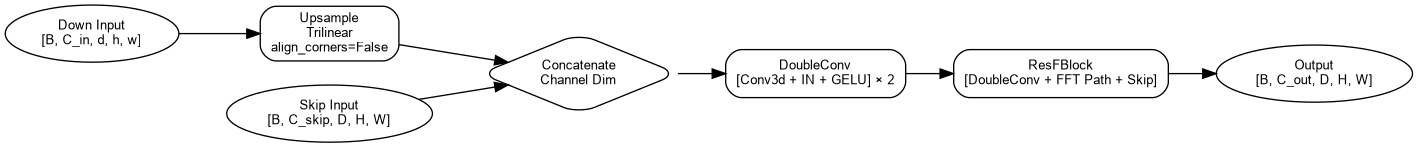
\includegraphics[width=0.8\textwidth]{figures/fft_up_block_architecture.png}
    \caption*{(c) UpBlock}
    
    \caption{Кастомная FFT\_UNet модель и её основные блоки}
    \label{fft_unet}
\end{figure}

Поскольку тензоры дифракционных картин не являются локально связанными, актуально использование механизма внимания. Он позволит модели находить связи между не близколежащими отражениями. Так, был разработан трансформер XRD\_Transformer для нашей задачи (рис. \ref{XRDTrans}). 

\begin{figure}[H]
    \centering
    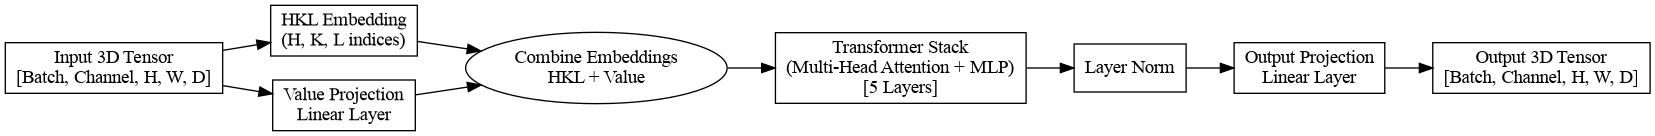
\includegraphics[width=1\textwidth]{figures/transformer.png}
    \caption{Архитектура модели XRD\_Transformer}
    \label{XRDTrans}
\end{figure}

В модели формируется единый эмбеддинг из эмбеддинга индексов Миллера (h,k,l) и проекции значений амплитуды отражений. Затем эмбеддинг подается в 5 слоев трансформера, которые состоят из Multi-Head Attention и полносвязного слоев. Затем после нормализации и обратного проецирования в исходное пространство получается восстановленный тензор дифракционной картины.

Так как нам известны все возможные значения индексов Миллера (h,k,l) эмбеддинг (рис. \ref{hklembed}) формируется следующим образом: каждый индекс кодируется one-hot энкодингом. Затем каждый вектор с помощью обучаемого линейного слоя проецируется к размерности embed\_dim/3; после конкатенации получается эмбеддинг позиции отражения размерности embed\_dim. Также в модели реализована возможность эмбеддинга через полносвязный слой, который проецирует позицию (h,k,l) сразу в вектор эмбеддинга, однако она не использовалась при обучении модели, так как первый способ является более физическим для нашей задачи, поскольку мы используем только симметрийно независимые отражения.


\begin{figure}[H]
    \centering
    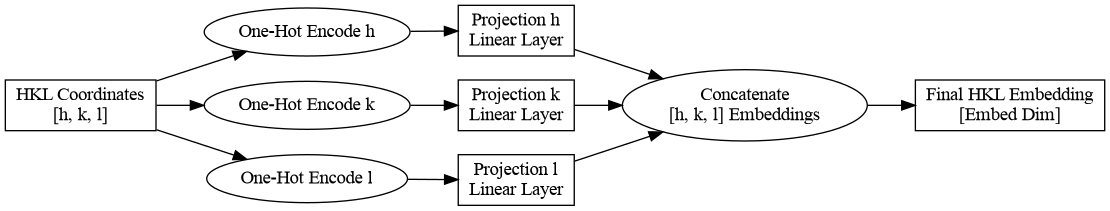
\includegraphics[width=1\textwidth]{figures/hkl_embedding_process.png}
    \caption{Схема формирования эмбеддинга HKL}
    \label{hklembed}
\end{figure}

В ходе выполнения работы также предложен постпроцессинг, включающий в себя учёт систематических погасаний --- "зануления" некоторых значений интенсивностей, что определяется симметрией структуры; в ходе обучения происходит явное восстановления части тензора, которую не нужно предсказывать.

Для обучения моделей UNet и FFT\_UNet использовался оптимизатор Adam с планировщиком plateau scheduler (обучение: learning rate = 0.01, factor = 0.1; дообучение: learning rate = 0.0001, factor = 0.5); для XRD\_Transformer --- оптимизатор AdamW с планировщиком cosine annealing (обучение: learning rate = 0.01; дообучение: learning rate = 0.0001).

В качестве функции потерь была выбрана среднеквадратичная ошибка, минимизация которой должна приводить к восстановлению тензора рентгеновских отражений. В качестве метрики для анализа используется R-фактор: $R = \frac{\sum |F_{obs} - F_{calc}|}{\sum |F_{obs}|}$, где $|F_{obs}|$ --- экспериментальные структурные факторы, $|F_{calc}|$ --- рассчитанные структурные факторы. R-фактор является общепринятым стандартом в кристаллографическом сообществе для оценки качества структурных моделей. Нулевое значение R-фактора отвечает идеальному соответствию между данными модельной структуры и экспериментальными данными.

Также в качестве метрики рассматривался SSIM, однако эксперименты с ним в качестве добавки к функции потери привели к более низкому качеству восстановления модели с точки зрения R-фактора. Данный результат можно объяснить отсутствием локальности наших данных.

Эффективность предсказания обученных моделей глубокого обучения проверялась на тестовой части синтетического датасета, а также тестовой части рентгенодифракционных данных моноклинных структур из CSD.
